\chapter{Migrace aplikace do kontejnerové virtualizace}
Kubernetes je funkční napříč různými platformami, od cloudu až po bare matel. V této práci je orchestrátor Kubernetes nainstalován přímo na fyzické servery, jejichž specifikace jsou uvedeny v tabulce \ref{tbl:hp_hardware}. Na všech serverech je nainstalován operační systém Ubuntu 16.04 pomocí open source nástroje Ubuntu MAAS.

\begin{table}[H]
\begin{center}
\caption{HW konfigurace HP serverů}
\label{tbl:hp_hardware}
\begin{tabular}{|l|l|}
\hline
\textbf{CPU} & Intel(R) Xeon(R) CPU E3-1231 v3 @ 3.40GHz (8 jader)\\
\hline
\textbf{RAM} & 32GB(4x 8GB) ECC DDR3 1600MHz \\
\hline
\textbf{HDD} & 2000GB (2x 1TB)  SATA 3.5" \\
\hline
\textbf{OS} & Ubuntu 16.04 LTS "Xenial Xerus" \\
\hline
\end{tabular}
\end{center}
\end{table}


\section{Instalace Kubernetes}
Jedním z důležitých faktorů je volba nástroje, pomocí kterého je Kubernetes cluster nainstalován, na trhu existuje celá řada takových nástrojů určených k instalaci. Tato řešení bývají většinou postavena okolo nástrojů na konfigurační management. Kubernetes cluster a kontejnery jsou prostředí, která jsou potřeba během používání řídit. Při výběru instalačního nástroje je také vhodné vyzkoušet, jakým způsobem  pracuje nástroj s koncepty LCM a jak je pomocí něj schopen řešit aktualizace samotného Kubernetes.

V této práci byl pro instalaci zvolen nástroj kargo, který se nachází pod hlavičkou kubernetes-incubátoru. Předností tohoto projektu je použití a implementace, je možné jej využit na instalaci Kubernetes clusteru napříč širokým spektrem cloudových prostředí, jako jsou AWS, GCE, OpenStack atd. Instalační nástroj kargo je postaven nad konfiguračním nástrojem Ansible, jeho použití je velmi jednoduché. Pro instalaci lze využít buď nástroj kargo-cli nebo přímo Ansible playbook s definicí pro cluster. Z důvodu nefunkčnosti nástroje kargo-cli je pro tuto práci zvoleno druhé řešení, instalace pomocí playbooku.

V rámci této práce není důležitá podrobná analýza karga. Pro demonstraci instalace stačí pouze inventory soubor, viz překlad kódu \ref{lst:kargo_invenotry}, do kterého je potřeba vyplnit ip adresy serverů a zvolit jednotlivé role. Pokud není při instalaci specifikováno síťové řešení, je kargo nainstalované s projektem Calico, což je jednoduché SDN řešení.

\begin{lstlisting}[caption={Inventory soubor pro Kargo},label={lst:kargo_invenotry}]
[kube-master]
10.0.175.86

[etcd]
10.0.175.86

[kube-node]
10.0.175.85
10.0.175.84
10.0.175.83

[k8s-cluster:children]
kube-node
kube-master
\end{lstlisting}

Po správném vyplnění inventory souboru stačí jen spustit daný Ansible playbook. \textit{Ansible-playbook -i inventory/inventory.cfg cluster.yml}.
Pokud není specifikován atribut flag \textit{-u} pro uživatele, Ansible se automaticky napojí na uživatele root. A po ssh se začne spojovat s ostatními servery a aplikovat proces nadefinovaný v Anible playbook. Užitečná vlastnost těchto konfiguračních nástrojů je idempotentnost. Pokud je přidán další server a znovu spuštěn playbook,  Ansible vyhodnotí, že na jednotlivých serverech je správná konfigurace. Pak na těchto serverech není v konfiguraci provedena žádná změna a instalace se spustí pouze na nově přidaných serverech.


Úspěšném dokončení instalace Kuberenetes pomocí karga lze zkontrolovat pomocí nástroje kubectl. Pomocí kubectl je možno zobrazit všechna zařízení zapojená do Kubernetes clusteru, viz ukázka kódu \ref{lst:kube_node}.

\begin{lstlisting}[caption={Kubernetes seznam node},label= {lst:kube_node}]
root@k8s-master:~/kargo# kubectl get nodes
NAME            STATUS                     AGE       VERSION
k8s-master      Ready,SchedulingDisabled   1m        v1.6.1+coreos.0
k8s-minion-01   Ready                      1m        v1.6.1+coreos.0
k8s-minion-02   Ready                      1m        v1.6.1+coreos.0
\end{lstlisting}

Po zobrazení seznamu podů v Kubernetes clusteru, obrázek \ref{lst:pods}, je zřejmé, že veškerý control plane Kubernetes je spuštěn taktéž v kontejnerech. Pokud není specifikován runtime, kargo spustí control plane v Docker kontejnerech.

\begin{lstlisting}[caption={Seznam podů po nainstalovaní Kuberentes},label= {lst:pods}]
root@k8s-master:~/kargo# kubectl get pods --all-namespaces
NAMESPACE     NAME                                  READY     STATUS    RESTARTS   AGE
kube-system   dnsmasq-624519416-1hx91               1/1       Running   0          1m
kube-system   dnsmasq-autoscaler-3605072793-q633q   1/1       Running   0          1m
kube-system   kube-apiserver-k8s-master             1/1       Running   0          1m
kube-system   kube-controller-manager-k8s-master    1/1       Running   0          1m
kube-system   kube-proxy-k8s-master                 1/1       Running   0          1m
kube-system   kube-proxy-k8s-minion-01              1/1       Running   0          1m
kube-system   kube-proxy-k8s-minion-02              1/1       Running   0          1m
kube-system   kube-scheduler-k8s-master             1/1       Running   0          1m
kube-system   kubedns-1519522227-8hhpl              3/3       Running   0          1m
kube-system   kubedns-autoscaler-1428750645-dttl6   1/1       Running   0          1m
kube-system   nginx-proxy-k8s-minion-01             1/1       Running   0          1m
kube-system   nginx-proxy-k8s-minion-02             1/1       Running   0          1m
\end{lstlisting}


\section{Sestavení kontejnerů}
Pro sestavení zdrojového image pro Docker kontejnery je nutné vytvořit Dockerfile. Dockerfile je jednoduchý soubor, s nímž se pracuje velmi podobně jako s bash skriptem. Tento soubor má několik klíčových příkazů, pomocí kterých se definují akce, které se při stavbě kontejneru spouští. Mohou zde být jisté podobnosti s klasickým Makefilem. 


\subsection{Příprava Dockerfile}
\label{sec:priprava}
Pro většinu komponent aplikace převáděné do kontejnerového prostředí je nutné připravit Dockerfile. Dockerfile je soubor, pomocí kterého je sestavena image na spuštění kontejneru. Pro správné použití je definován seznam doporučených pravidel, která by měl každý Dockerfile před tvorbou image splňovat. Tato pravidla byla aplikovaná i v této práci.

Kontejnery by měly mít co nejmenší velikost, definice v Dockerfile by měla být co nejstručnější a neměly by zde být žádné závislosti na nepotřebných balících. V případě nutnosti musí být možné kontejner zastavit, smazat či znovu spustit jen bez úpravy konfigurace.
%https://12factor.net/processes

Při instalaci balíčku je vhodné vyloučit balíky, které nikdy nebudou použity a které by ovlivňovaly velikost kontejneru. Například textové editory jako vim, nano, atd. do kontejnerů nepatří.

Každý kontejner by měl vykonávat pouze jednu činnost, na kterou je zaměřen. Pokud je tato podmínka splněna, kontejnery lze horizontálně škálovat. Jeli možno samostatnou aplikaci rozložit na několik částí, je dobré z nich vytvořit samostatné kontejnery.

V každé image je důležité minimalizovat počet vrstev. I přesto že Docker dokáže pracovat až s 127 vrstvami, je vhodné najít rovnováhu mezi přehledností. V případě použití příliš mnoha vrstev je nutno vrstvy slučovat a sestavit celý image znovu. Ne ve všech případech je vhodné sestavovat novou image, lze použít i image z veřejného repositáře. Na těchto repositářích se nachází spousta images, které byly sestaveny uživateli. Bohužel uživatelé většinou nepřidávají žádné Readme (popis image) nebo Dockerfile, podle kterého byla image sestavena. Je tak nebezpečné ji použít z důvodu možnosti existence škodlivého softwaru. V konceptu vrstev hlavní myšlenkou je, že právo na zapisovaní má pouze vrchní vrstva\cite{Docker_learning}. Pokud je nutné provést úpravy v read-only vrstvě, pak je daný soubor přesunut na vrchní vrstvu a upraven zde. Demonstrace Dockerfile je předvedena na předpisu pro MySql cluster.

První řádek každého Dockerfile začíná klíčovým slovem \textbf{FROM}. Tento řádek určuje, jaká image bude základem. Ve většině případů se používají Linuxové distribuce jako Ubuntu, Centos, Debian, atd. Výběr této základní image bývá často podceňován a v drtivé většině případů je vybrán systém Ubuntu. Problém klasických distribucí je styl doručování. V základních image obsahují spoustu nepotřebných balíčků, které zvětšují velikost kontejnerů. Nástroje z těchto balíčků nejsou v kontejneru vůbec využity. Řešením  problému je použití speciálních distribucí, které doručují čisté Linuxové jádro bez ovladačů a dalších přidaných nástrojů. Vhodné je použít například Alpine Linux, který má velikost pouze 6 MB i s vlastním balíčkovacím systémem. Dalším kritériem je rychlost sestavení, čím větší image, tím je delší doba potřebná pro sestavení image. Pokud je použit Alpine Linux, je sestavení o více než 15 vteřin rychlejší než na Ubuntu\cite{ubuntu_alpine}. V úvodní části je také vhodné nastavit proměnné pomocí \textbf{ENV} a argumentů \textbf{ARG} hodnoty pro proměnné. To pomůže při aktualizaci a stavbě nových kontejnerů. V této práci jsou v argumentech uloženy specifické verze balíků, které se mají do výsledného image nainstalovat.

Při tvorbě uvedeného image nebyl použit Alpine Linux, je to jediná část z migrované aplikace postavená na klasické distribuci. Důvod je jednoduchý, balíčky pro galera cluster jsou dostupné pouze ve formě Debian package.

\begin{lstlisting}[caption={Dockerfile, část 1.},label= {lst:df1}]
FROM debian:jessie

ARG galera_version=3
ARG mysql_version=5.6

ENV GALERA_VERSION $galera_version
ENV MYSQL_VERSION $mysql_version

\end{lstlisting}


V Dockerfile je důležité minimalizovat počet všech použitých příkazů. Problematika vrstev v Dockefile byla popsána v části \ref{sec:priprava} Pomocí  \textbf{RUN} lze spouštět jednotlivé příkazy v shellu. Příkazy jsou odděleny pomocí \textit{\&\&} a \textit{$\backslash$}, při sestavování pak Docker vyhodnotí, že se jedná o jeden řádek, viz ukázka kódu \ref{lst:df1}. Proto vytvoří pouze jednu vrstvu v tomto případě pro aktualizaci repositářů a přidání GPG klíčů pro repositáře.

\begin{lstlisting}[caption={Seznam podů po nainstalovaní Kuberentes},label= {lst:pods}]
RUN     apt-key adv --keyserver keyserver.ubuntu.com --recv-keys 8507EFA5 && \
        apt-key adv --keyserver keyserver.ubuntu.com --recv-keys BC19DDBA && \

        echo "deb http://releases.galeracluster.com/debian jessie main" > /etc/apt/sources.list.d/galera.list && \
        echo "deb http://repo.percona.com/apt jessie main" > /etc/apt/sources.list.d/percona.list && \

\end{lstlisting}

Pro přehlednost je také nutno rozdělovat \textbf{RUN} příkazy do logických bloků. Z ukázky kódu \ref{lst:df2} je patrné přidání MySql uživatelů a instalace samostatných balíčků, ve kterých je specifikovaná konkrétní verze, která je uvedená pomocí odkazů na argumenty definované ve vrchní části uvedeného Dockerfile. Akce, které se budou často měnit, je správné uvést na konec Dockerfile, Docker pak rozpozná, že změna se týká pouze dané části, a spustí tak proces sestavování až od výskytu změny.

\begin{lstlisting}[caption={Dockerfile, část 2},label= {lst:df2}]


RUN groupadd -r mysql && useradd -r -g mysql mysql

RUN apt-get update && \
    DEBIAN_FRONTEND=nointeractive apt-get -y install galera-${GALERA_VERSION} galera-arbitrator-${GALERA_VERSION} mysql-wsrep-${MYSQL_VERSION} mysql-wsrep-server-${MYSQL_VERSION} percona-xtrabackup percona-toolkit libdbd-mysql-perl rsync netcat-openbsd netcat && \
    rm -rf /var/lib/mysql/* && \
    apt-get clean && rm -rf /var/lib/apt/lists/* /tmp/* /var/tmp/*
\end{lstlisting}

Prostřednictvím \textbf{ENTRYPOINT} lze nastavit sadu příkazů a vstupů, které mají být podsunuty do kontejneru během jeho startu. V případě této image jsou entrypointy určovány externím souborem obsahujícím bashový script, který si po vložení parametru MYSQL\_ROOT\_PASSWORD vytvoří uživatele root s tímto heslem. Jsou zde řešena především nastavení pro clusterování databáze. Pomocí příkazu \textbf{EXPOSE} lze Docker kontejneru nařídit, na kterém specifickém portu má poslouchat, když je spuštěn, viz ukázka kódu \ref{lst:df3}. Pokud žádná služba uvnitř kontejneru neposlouchá na daném portu, Docker port zvenku uzavře.

\begin{lstlisting}[caption={Dockerfile, část 3},label= {lst:df3}]
COPY files/entrypoint.sh /entrypoint.sh
ENTRYPOINT ["/entrypoint.sh"]`'
RUN chmod +x /entrypoint.sh

EXPOSE 3306 4444 4567 4568

\end{lstlisting}


\subsection{Sestavení  kontejnerů a upload na Docker Hub}
Sestavení Docker kontejneru probíhá pomocí vestavěného nástroje \textit{build}, kterému stačí předat správnou cestu k Dockerfile. Soubor, ze kterého se bude image stavět, musí mít název Dockerfile. Pokud je Dockerfile správně napsaný, Docker automaticky provede všechny procesy v něm stanovené. Po úspěšném sestavení je vhodné daný image otagovat. Pokud není stanoveno, image si nastaví tag jako latest, ale to není ve všech případech vhodné, například u aplikací, které se během času vyvíjejí. Sestavený image je vidět na ukázce kódu \ref{docker:iamges}

\begin{lstlisting}[caption={Seznam neotagovaných Docker Image po vytvoření},label= {docker:images}]
root@Thorfinn:/home/lotharkatt/thesis/galera# docker images
REPOSITORY                   TAG                 IMAGE ID            CREATED             SIZE
galera                       latest              c4da48070bb7        16 seconds ago      548 MB
\end{lstlisting}

Pokud je image vystaven na veřejném repositáři, bude dostupný pro kohokoliv, viz obrázek \ref{fig:docker_repository}. V práci je využit veřejný repositář Docker hub. Před nahráváním je nutné změnit tag a do jména přidat uživatelský namepsace, pod kterým se bude daná image nahrávat do repositáře. Image se na repositář nahraje pomocí příkazu Docker \textit{push}.

\begin{figure}[H]
\begin{centering}
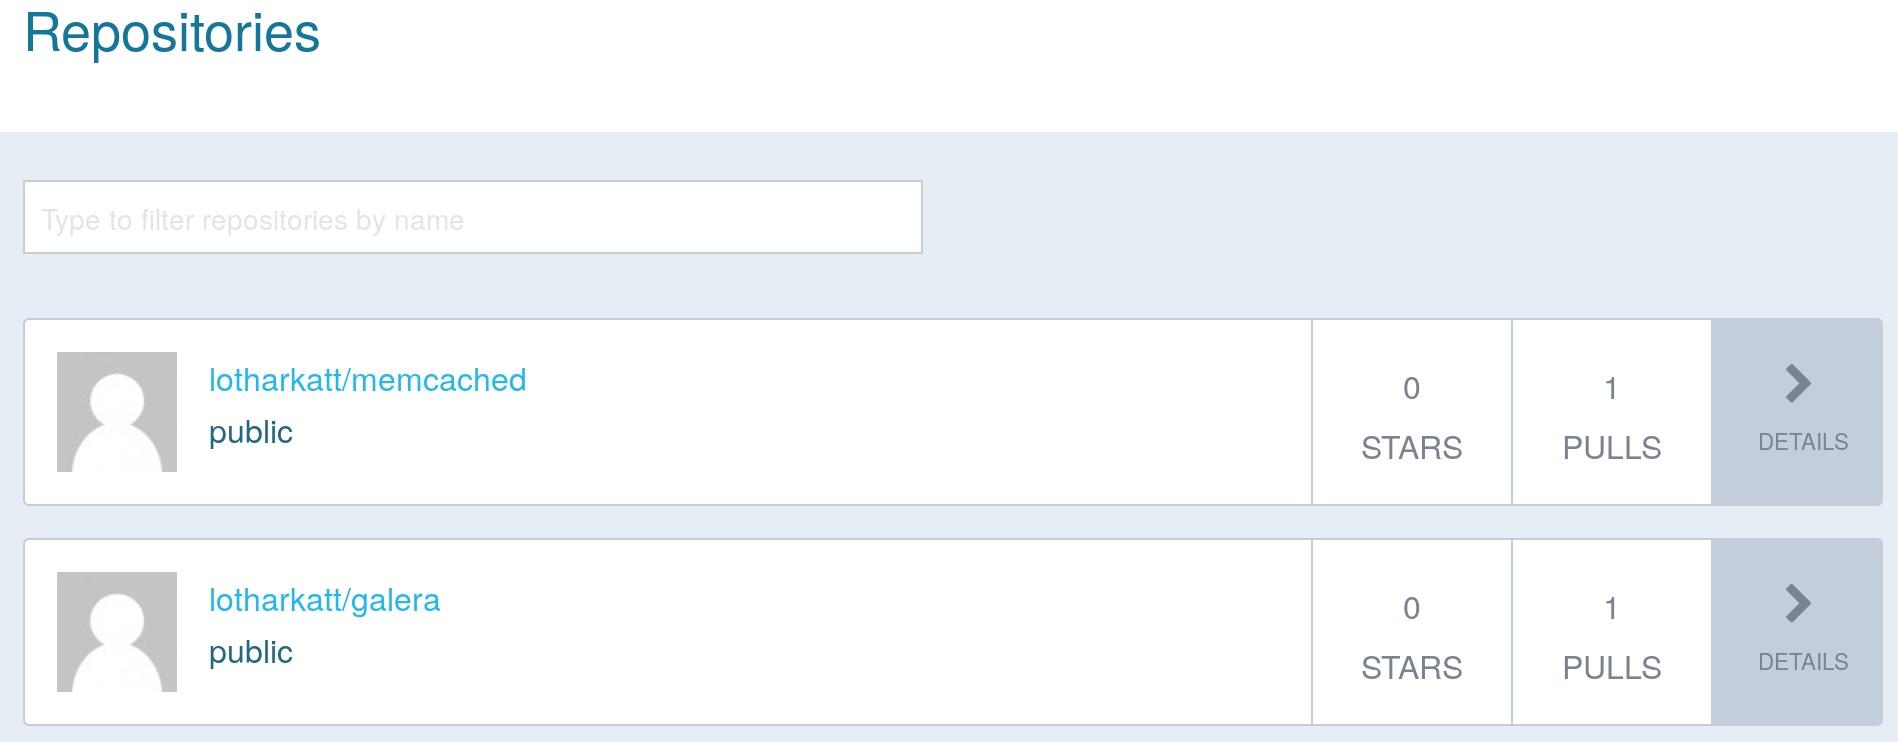
\includegraphics[width=1.0\textwidth]{img/docker_repository}
\par\end{centering}
\caption{Image nahrané na Docker Hub, zdroj: vlastní tvorba \label{fig:docker_repository}}
\end{figure}


\section{Kubernetes}
Pro nasazení kontejnerů do orchestrátoru je nutno napsat konfigurační soubor v formátu yaml. Všechny komponenty Kubernetes se dají nadefinovat pomocí yaml souborů. Pro přehlednost a přístupnost je nutné jednotlivé komponenty a aplikace sdružovat do skupin pomocí namespaců. Pomocí namespacu lze také přidělovat práva jednotlivým uživatelům přistupujícím do Kubernetes clusteru. Je nežádoucí, aby všichni uživatelé měli přístup ke všem aplikacím běžícím na jedné infrastruktuře. Jednotlivé komponenty se zobrazují pomocí přepínače \textit{--namespace <název namespace>}. V této práci tento způsob označování aplikace využit nebyl z důvodu běhu pouze jedné aplikace v Kubernetes clusteru. Celý konfigurační soubor je vysvětlen na ukázce kódu \ref{lst:k8s-1}.

\begin{lstlisting}[caption={Ukázka konfigurace Kubernetes  komponent, část 1},label= {lst:k8s-1}]
---
apiVersion: v1
kind: Namespace
metadata:
  name: web-application
---
\end{lstlisting}

Kubernetes service lze nazvat jako sdružení pravidel, která spojují pody navzájem. Kromě metadat jako je jméno a label, se musí specifikovat porty, přes které budou aplikace dostupné. V případě vzorového kódu \ref{lst:k8s-2} se jedná o port 3306. Pomocí této definice bude port 3306 nastaven kontejnerům uvnitř podu. 

\begin{lstlisting}[caption={Ukázka konfigurace Kubernetes komponent, část 2},label= {lst:k8s-2}]
kind: Service
apiVersion: v1
metadata:
  name: mysql
  labels:
    name: mysql
spec:
  ports:
    - name: mysql
      port: 3306
      protocol: TCP
  selector:
name: mysql
\end{lstlisting}

Deploymentem by se dala označit obecná definice podů. Definice deploymentu určuje, kolik replik a jakou image má obsahovat. Na základně této definice vzniká ReplicaSet (Replication Controller), pomocí kterého se škálují kontejnery. Z ukázky číslo \ref{lst:k8s-3} je vidět základní definici podu. Tato konfigurační část začíná specifikací počtu replik, které budou vytvořené po spuštění yamlu s předpisem pro deployment. Následuje definice pro kontejner,  nastavení image. V základním nastavení je image stahován z veřejného repositáře Docker Hub. Zde je nutné poznamenat, že pokud je vyžadována specifická verze image jako v této práci, je nutné za cestu k image také uvést správnou verzi, jinak kontejner nebude správně spuštěn. Dalším důležitým parametrem je port, který má být pro pod otevřen. V práci se jedná o port 3306, port pro MySql databázi. Poté následuje deklarace enviromentalních proměnných, které jsou vyžadovány pro správný běh databáze. Celá definice je zakončena VolumemMountem. Pomocí této definice je nastaveno, že veškerý obsah adresáře \textit{/var/lib/mysql/} bude přesunut na hostitelský systém do cesty \textit{/home/ubuntu/mysql/}. Pokud by nebyla cesta z kontejneru nadefinovaná, aplikace by po pádu kontejneru přišla o veškerá data. 

\begin{lstlisting}[caption={Ukázka konfigurace Kubernetes komponent, část 3},label= {lst:k8s-3}]
apiVersion: extensions/v1beta1
kind: Deployment
metadata:
  name: mysql
spec:
  replicas: 1
  template:
    metadata:
      labels:
        name: mysql
    spec:
      containers:
      - image: lotharkatt/galera:1.0
        name: mysql
        ports:
        - containerPort: 3306
        env:
        - name: MYSQL_DATABASE
          value: owncloud_db
        - name: MYSQL_USER
          value: admin
        - name: MYSQL_PASSWORD
          value: password 
        volumeMounts:
        - mountPath: /var/lib/mysql/
          name: mysql
      volumes:
        - hostPath:
            path: /home/ubuntu/mysql/
	      name: mysql
\end{lstlisting}

Vytvoření podů pak probíhá zavoláním příkazu \textit{kubectl create -f <cesta k konfiguračnímu yaml souboru>}.  Při spuštění uvedeného Kubernetes konfiguračního souboru pro mysql se spustí dvě komponenty, deployment a service. Součástí deploymentu je také ReplicaSet. Pokud je konfigurace vyplněná správně, při zobrazení listu služeb, bude vyexportován daný port.

Klíčovou vlastnost, kterou je potřeba pro Kubernetes cluster nakonfigurovat, je viditelnost vůči venkovním sítím. Orchestrátor si adresuje pody nezávisle na síťových rozsazích. Pro dostupnost sítí z vnějšího světa lze použít hned několik způsobů přístupu. Nejjednoduší je konfigurace parametru NodePort, pomocí kterého lze vyexportovat port podu přímo na port hostitelského stroje. Tento postup byl použit v této práci. Další možností je nastavení tzv. kube-proxy, jak už název napovídá, jedná se o proxy řešení, přes které lze přistupovat rovněž do venkovní sítě. Pro komunikaci s venkovní sítí také lze použít komponentu ingress, přes kterou je možné přistupovat přímo na servisní porty. 

\subsection{Ukázka škálování}
Kubernetes podporuje horizontální škálování, v následující ukázce kódu \ref{lst:scale-1} je zobrazen výpis jednotlivých podů s jejich stavem. Je vidět, že jednotlivé pody mají alokované IP adresy, které jim přiřadil sám orchestrátor, a fyzická zařízení, na která je umístil scheduler. Automatické adresování kontejnerů je důležité zejména díky škálování, není možné, aby při přidávaní kontejnerů administrátor hlídal adresní rozsahy a adresoval pody ručně. 

\begin{lstlisting}[caption={Ukázka škálování, čast 1},label= {lst:scale-1}]
root@k8s-master:~# kubectl get pods -o wide
NAME                         READY     STATUS    RESTARTS   AGE       IP              NODE
memcached-3034518848-hhpz3   1/1       Running   0          4m        10.233.76.116   k8s-minion-02
mysql-1155545570-1rnms       1/1       Running   0          10m       10.233.76.113   k8s-minion-02
nginx-3571296254-2fkjm       1/1       Running   0          7m        10.233.76.115   k8s-minion-02
owncloud-4254227122-37qfs    1/1       Running   0          23s       10.233.95.54    k8s-minion-01
\end{lstlisting}

Pro zobrazení aktuálního počtu a stavu lze použít deployment list, který zobrazuje aktuální počet jednotlivých podů. Kromě počtu a dostupnosti podů je zde sloupec up-to-date, který při spuštění rolling updatu ukazuje počet aktualizovaných podů. Seznam deploymentů je zobrazen v ukázce kódu \ref{lst:scale-2}

\begin{lstlisting}[caption={Ukázka škálování, čast 2},label= {lst:scale-2}]
root@k8s-master:~# kubectl get deployment 
NAME        DESIRED   CURRENT   UP-TO-DATE   AVAILABLE   AGE
memcached   1         1         1            1           5m
mysql       1         1         1            1           11m
nginx       1         1         1            1           8m
owncloud    1         1         1            1           1m
\end{lstlisting}

Pro vyvolání škálovaní se používá příkaz kubectl, přes který se ovládá celý Kubernetes cluster. Pomocí příkazu {\textit{kubectl scale deployment/owncloud --replicas=5} se vyškálují pody s kontejnery na stanovenou hodnotu, v tomto případě se jedná o pět replik. Proces replikace probíhá následovně: je změněna hodnota replik, ta je odeslána přes API server na ReplicaSet (Replication Controller), ten zavolá scheduler a pošle mu požadovaný počet nových podů, scheduler je pak vytvoří na nodech, kde jsou dostupné zdroje. Škálování podů probíhá paralelně, je spouštěno několik replik najednou. Výsledek vyškálované aplikace je zobrazen na ukázce kódu \ref{lst:scale-3}

\begin{lstlisting}[caption={Ukázka škálování, čast 3},label= {lst:scale-3}]
root@k8s-master:~# kubectl get deployment  
NAME        DESIRED   CURRENT   UP-TO-DATE   AVAILABLE   AGE
memcached   1         1         1            1           7m
mysql       1         1         1            1           13m
nginx       1         1         1            1           9m
owncloud    5         5         5            5           2m
\end{lstlisting}

Pro ověření úspěšného škálování je vhodné zkontrolovat seznam podů, na ukázce kódu \ref{lst:scale-4} lze vidět, že všechny kontejnery byly úspěšně vyškálovány bez jakéhokoliv pádu či restartu. Při srovnání s ukázkou kódu \ref{lst:scale-1} je možno vidět, že původní pod s kontejnery aplikace OwnCloud zůstal nezměněn. 

Pro automatické škálovaní, které v této práci nebude demonstrováno, lze použít jednoduchý předpis buď pro Replication Controller, nebo přímo deployment. Například {\textit{kubectl autoscale deployment owncloud --min=2 --max=5 --cpu-percent=60}, pomocí tohoto příkazu se začne pod automaticky škálovat, jakmile hranice vytížení procesoru kontejneru stoupne nad 60 procent do počtu stanovených replik. Toto je výhodné při velkém vytížení webové aplikace, pokud do ní přistupuje mnoho uživatelů, aplikace se sama automaticky naškáluje. Jakmile zátěž procesoru poklesne, počet podů s kontejnery se opět sníží.

\begin{lstlisting}[caption={Ukázka škálování, čast 4},label= {lst:scale-4}]
root@k8s-master:~# kubectl get pods -o wide
NAME                         READY     STATUS    RESTARTS   AGE       IP              NODE
memcached-3034518848-hhpz3   1/1       Running   0          7m        10.233.76.116   k8s-minion-02
mysql-1155545570-1rnms       1/1       Running   0          13m       10.233.76.113   k8s-minion-02
nginx-3571296254-2fkjm       1/1       Running   0          9m        10.233.76.115   k8s-minion-02
owncloud-4254227122-37qfs    1/1       Running   0          2m        10.233.95.54    k8s-minion-01
owncloud-4254227122-9190b    1/1       Running   0          14s       10.233.76.117   k8s-minion-02
owncloud-4254227122-gmpp8    1/1       Running   0          14s       10.233.95.55    k8s-minion-01
owncloud-4254227122-n77pv    1/1       Running   0          14s       10.233.76.118   k8s-minion-02
owncloud-4254227122-v6dg0    1/1       Running   0          14s       10.233.95.56    k8s-minion-01
\end{lstlisting}

\subsection{Vysoká dostupnost}
Demonstrace vysoké dostupnosti byla provedena na ukázce již naškálované aplikace. Na ukázce kódu \ref{lst:trouble-1} je zobrazen seznam podů před ukázkou vysoké dostupnosti. 

V této ukázce bude z Kubernetes clusteru vyřazen jeden fyzický sever, který slouží jako minion pro běh podů. Výpadek serveru označen jako k8s-minion-01 bude proveden pomocí tvrdého vypnutí serveru přímo přes ILo daného fyzického zařízení.

\begin{lstlisting}[caption={Seznam podů po nainstalovaní Kuberentes},label= {lst:trouble-1}]
root@k8s-master:~# kubectl get pods -o wide
NAME                         READY     STATUS    RESTARTS   AGE       IP              NODE
memcached-3034518848-hhpz3   1/1       Running   0          10m       10.233.76.116   k8s-minion-02
memcached-3034518848-hmvl0   1/1       Running   0          55s       10.233.76.120   k8s-minion-02
memcached-3034518848-vcpgk   1/1       Running   0          55s       10.233.95.59    k8s-minion-01
mysql-1155545570-1rnms       1/1       Running   0          16m       10.233.76.113   k8s-minion-02
mysql-1155545570-647b7       1/1       Running   0          1m        10.233.76.119   k8s-minion-02
mysql-1155545570-7dpg9       1/1       Running   0          1m        10.233.95.58    k8s-minion-01
nginx-3571296254-2fkjm       1/1       Running   0          13m       10.233.76.115   k8s-minion-02
nginx-3571296254-hpnpd       1/1       Running   0          1m        10.233.95.57    k8s-minion-01
owncloud-4254227122-9190b    1/1       Running   0          3m        10.233.76.117   k8s-minion-02
owncloud-4254227122-n77pv    1/1       Running   0          3m        10.233.76.118   k8s-minion-02
\end{lstlisting}

Po vypnutí miniona rozeznal Kubernetes cluster, že minion je nedostupný. V základním nastavení je reakční doba pět minut. Po uplynutí této doby jsou všechny instance z nedostupného nodu přemigrovány na zbylé miniony. Tento fakt je znázorněn na ukázce kódu \ref{lst:trouble-2}. Pody jsou vytvořeny s odlišným jménem a subnetem odpovídajícím rozsahu druhého nodu.

Tento koncept dodává vysokou flexibilitu a dostupnost jednotlivých služeb. Tento proces funguje správně jen díky bezstavovému modelu aplikací, které nejsou v důsledku závislé na hostitelském systému.

\begin{lstlisting}[caption={Seznam podů po nainstalovaní Kuberentes},label= {lst:trouble-2}]
root@k8s-master:~# kubectl get pods -o wide
NAME                         READY     STATUS             RESTARTS   AGE       IP              NODE
memcached-3034518848-69rwq   1/1       Running            0          23m       10.233.76.121   k8s-minion-02
memcached-3034518848-hhpz3   1/1       Running            0          40m       10.233.76.116   k8s-minion-02
memcached-3034518848-hmvl0   1/1       Running            0          30m       10.233.76.120   k8s-minion-02
mysql-1155545570-1rnms       1/1       Running            0          46m       10.233.76.113   k8s-minion-02
mysql-1155545570-647b7       1/1       Running            0          30m       10.233.76.119   k8s-minion-02
mysql-1155545570-vsbd6       1/1       Running            0          23m       10.233.76.122   k8s-minion-02
nginx-3571296254-2fkjm       1/1       Running            0          42m       10.233.76.115   k8s-minion-02
nginx-3571296254-rrm2n       1/1       Running            0          23m       10.233.76.123   k8s-minion-02
owncloud-4254227122-9190b    1/1       Running            0          33m       10.233.76.117   k8s-minion-02
owncloud-4254227122-n77pv    1/1       Running            0          33m       10.233.76.118   k8s-minion-02
\end{lstlisting}